\XtoCBlock{Average}
\label{block:Average}
\begin{figure}[H]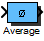
\includegraphics{Average}\end{figure} 

\begin{XtoCtabular}{Inports}
In & Input value\tabularnewline
\hline
\end{XtoCtabular}


\begin{XtoCtabular}{Outports}
Out & Averaged value\tabularnewline
\hline
\end{XtoCtabular}

\begin{XtoCtabular}{Mask Parameters}
n & Number of points to be averaged over\tabularnewline
\hline
ts\_fact & Multiplication factor of base sampling time (in integer format)\tabularnewline
\hline
\end{XtoCtabular}

\subsubsection*{Description:}
Calculation of moving average value over n numbers.

% include optional documentation file
\InputIfFileExists{\XcHomePath/Library/Math/Doc/Average_Info.tex}{\vspace{1ex}}{}

\subsubsection*{Implementations:}
\begin{tabular}{l l}
\textbf{FiP8} & 8 Bit Fixed Point Implementation\tabularnewline
\textbf{FiP16} & 16 Bit Fixed Point Implementation\tabularnewline
\textbf{FiP32} & 32 Bit Fixed Point Implementation\tabularnewline
\textbf{Float32} & 32 Bit Floating Point Implementation\tabularnewline
\textbf{Float64} & 64 Bit Floating Point Implementation\tabularnewline
\end{tabular}

\XtoCImplementation{FiP8}
\index{Block ID!5024}
\nopagebreak[0]
% Implementation details
\begin{tabular}{l l}
\textbf{Name} & FiP8 \tabularnewline
\textbf{ID} & 5024 \tabularnewline
\textbf{Revision} & 1 \tabularnewline
\textbf{C filename} & Average\_FiP8.c \tabularnewline
\textbf{H filename} & Average\_FiP8.h \tabularnewline
\end{tabular}
\vspace{1ex}

8 Bit Fixed Point Implementation

\begin{XtoCtabular}{Controller Parameters}
n & Average window size\tabularnewline
\hline
sfrn & Shift factor for computation of average value sfrn = ld(n)\tabularnewline
\hline
sum & Temporary sum\tabularnewline
\hline
count & Index counter\tabularnewline
\hline
avg & Array with data values\tabularnewline
\hline
\end{XtoCtabular}

% Implementation data structure
\XtoCDataStruct{Data Structure:}
\begin{lstlisting}
typedef struct {
     uint16        ID;
     int8          *In;
     int8          Out;
     uint16        n;
     uint8         sfrn;
     int16         sum;
     uint16        count;
     int8          *avg;
} AVERAGE_FIP8;
\end{lstlisting}

\ifdefined \AddTestReports
\InputIfFileExists{\XcHomePath/Library/Math/Doc/Test_Average_FiP8.tex}{}{}
\fi
\XtoCImplementation{FiP16}
\index{Block ID!5025}
\nopagebreak[0]
% Implementation details
\begin{tabular}{l l}
\textbf{Name} & FiP16 \tabularnewline
\textbf{ID} & 5025 \tabularnewline
\textbf{Revision} & 1 \tabularnewline
\textbf{C filename} & Average\_FiP16.c \tabularnewline
\textbf{H filename} & Average\_FiP16.h \tabularnewline
\end{tabular}
\vspace{1ex}

16 Bit Fixed Point Implementation

\begin{XtoCtabular}{Controller Parameters}
n & Average window size\tabularnewline
\hline
sfrn & Shift factor for computation of average value sfrn = ld(n)\tabularnewline
\hline
sum & Temporary sum\tabularnewline
\hline
count & Index counter\tabularnewline
\hline
avg & Array with data values\tabularnewline
\hline
\end{XtoCtabular}

% Implementation data structure
\XtoCDataStruct{Data Structure:}
\begin{lstlisting}
typedef struct {
     uint16        ID;
     int16         *In;
     int16         Out;
     uint16        n;
     uint8         sfrn;
     int32         sum;
     uint16        count;
     int16         *avg;
} AVERAGE_FIP16;
\end{lstlisting}

\ifdefined \AddTestReports
\InputIfFileExists{\XcHomePath/Library/Math/Doc/Test_Average_FiP16.tex}{}{}
\fi
\XtoCImplementation{FiP32}
\index{Block ID!5026}
\nopagebreak[0]
% Implementation details
\begin{tabular}{l l}
\textbf{Name} & FiP32 \tabularnewline
\textbf{ID} & 5026 \tabularnewline
\textbf{Revision} & 1 \tabularnewline
\textbf{C filename} & Average\_FiP32.c \tabularnewline
\textbf{H filename} & Average\_FiP32.h \tabularnewline
\end{tabular}
\vspace{1ex}

32 Bit Fixed Point Implementation

\begin{XtoCtabular}{Controller Parameters}
n & Average window size\tabularnewline
\hline
sfrn & Shift factor for computation of average value sfrn = ld(n)\tabularnewline
\hline
sum & Temporary sum\tabularnewline
\hline
count & Index counter\tabularnewline
\hline
avg & Array with data values\tabularnewline
\hline
\end{XtoCtabular}

% Implementation data structure
\XtoCDataStruct{Data Structure:}
\begin{lstlisting}
typedef struct {
     uint16        ID;
     int32         *In;
     int32         Out;
     uint16        n;
     uint8         sfrn;
     int64         sum;
     uint16        count;
     int32         *avg;
} AVERAGE_FIP32;
\end{lstlisting}

\ifdefined \AddTestReports
\InputIfFileExists{\XcHomePath/Library/Math/Doc/Test_Average_FiP32.tex}{}{}
\fi
\XtoCImplementation{Float32}
\index{Block ID!5027}
\nopagebreak[0]
% Implementation details
\begin{tabular}{l l}
\textbf{Name} & Float32 \tabularnewline
\textbf{ID} & 5027 \tabularnewline
\textbf{Revision} & 0.1 \tabularnewline
\textbf{C filename} & Average\_Float32.c \tabularnewline
\textbf{H filename} & Average\_Float32.h \tabularnewline
\end{tabular}
\vspace{1ex}

32 Bit Floating Point Implementation

\begin{XtoCtabular}{Controller Parameters}
n & Average window size\tabularnewline
\hline
sum & Temporary sum\tabularnewline
\hline
count & Index counter\tabularnewline
\hline
avg & Array with data values\tabularnewline
\hline
\end{XtoCtabular}

% Implementation data structure
\XtoCDataStruct{Data Structure:}
\begin{lstlisting}
typedef struct {
     uint16        ID;
     float32       *In;
     float32       Out;
     uint16        n;
     float32       sum;
     uint16        count;
     float32       *avg;
} AVERAGE_FLOAT32;
\end{lstlisting}

\ifdefined \AddTestReports
\InputIfFileExists{\XcHomePath/Library/Math/Doc/Test_Average_Float32.tex}{}{}
\fi
\XtoCImplementation{Float64}
\index{Block ID!5028}
\nopagebreak[0]
% Implementation details
\begin{tabular}{l l}
\textbf{Name} & Float64 \tabularnewline
\textbf{ID} & 5028 \tabularnewline
\textbf{Revision} & 0.1 \tabularnewline
\textbf{C filename} & Average\_Float64.c \tabularnewline
\textbf{H filename} & Average\_Float64.h \tabularnewline
\end{tabular}
\vspace{1ex}

64 Bit Floating Point Implementation

\begin{XtoCtabular}{Controller Parameters}
n & Average window size\tabularnewline
\hline
sum & Temporary sum\tabularnewline
\hline
count & Index counter\tabularnewline
\hline
avg & Array with data values\tabularnewline
\hline
\end{XtoCtabular}

% Implementation data structure
\XtoCDataStruct{Data Structure:}
\begin{lstlisting}
typedef struct {
     uint16        ID;
     float64       *In;
     float64       Out;
     uint16        n;
     float64       sum;
     uint16        count;
     float64       *avg;
} AVERAGE_FLOAT64;
\end{lstlisting}

\ifdefined \AddTestReports
\InputIfFileExists{\XcHomePath/Library/Math/Doc/Test_Average_Float64.tex}{}{}
\fi
